% =====================================================================
%  Ευφυή Συστήματα — 1η Εργασία: Ταξινόμηση IRIS με ασαφές μοντέλο TSK (ANFIS)
%  Πρότυπο: IEEE Conference (IEEEtran)
%
%  ΟΔΗΓΙΕΣ OVERLEAF:
%    1. New Project -> Upload -> ανέβασε αυτό το αρχείο + τον φάκελο figures/
%    2. Menu -> Compiler: LuaLaTeX   (ΟΧΙ pdfLaTeX — χρειάζεται για τα ελληνικά)
%  Αν βγει σφάλμα γραμματοσειράς: άλλαξε το "STIX Two Text" σε "FreeSerif".
% =====================================================================
\documentclass[conference]{IEEEtran}

\usepackage{fontspec}
\setmainfont{STIX Two Text}            % Times-like, με ελληνικούς χαρακτήρες
\setmonofont{FreeMono}                 % monospace με ελληνικά (αποφυγή σφάλματος polyglossia)
\usepackage{polyglossia}
\setdefaultlanguage{greek}
\setotherlanguage{english}

\usepackage{amsmath,amssymb}
\usepackage{graphicx}
\usepackage{booktabs}
\usepackage{cite}
\graphicspath{{figures/}}

\renewcommand{\IEEEkeywordsname}{Λέξεις-κλειδιά}

\begin{document}

\title{Ταξινόμηση του συνόλου δεδομένων IRIS\\με ασαφές μοντέλο Takagi--Sugeno--Kang (ANFIS)}

\author{\IEEEauthorblockN{Απόστολος Δαγκλής}
\IEEEauthorblockA{Τμήμα Μηχανικών Πληροφορικής και Ηλεκτρονικών Συστημάτων\\
Διεθνές Πανεπιστήμιο της Ελλάδος (ΔΙΠΑΕ)\\
Α.Μ.: 2021031 \quad daglisapo1@gmail.com}}

\maketitle

% ---------------------------------------------------------------------
\begin{abstract}
Η εργασία παρουσιάζει έναν ταξινομητή για τις τρεις κλάσεις του συνόλου δεδομένων
IRIS, βασισμένο σε ασαφές μοντέλο τύπου Takagi--Sugeno--Kang (TSK) πρώτης τάξης,
υλοποιημένο ως προσαρμοστικό νευρο-ασαφές σύστημα (ANFIS). Το μοντέλο έχει
τέσσερις εισόδους, δύο Gaussian συναρτήσεις συμμετοχής ανά είσοδο και 16 κανόνες
σε διαμέριση πλέγματος. Γράφτηκε από την αρχή σε Python/NumPy, χωρίς έτοιμες
βιβλιοθήκες ANFIS. Η εκπαίδευση είναι υβριδική: οι παράμετροι των
συμπερασμάτων υπολογίζονται με ελάχιστα τετράγωνα με κανονικοποίηση ridge
και οι παράμετροι των συναρτήσεων συμμετοχής προσαρμόζονται με κατάβαση κλίσης
σε αριθμητικά υπολογισμένη κλίση. Τα δεδομένα χωρίστηκαν τυχαία και
στρωματοποιημένα σε σύνολα Training/Checking/Testing (70/15/15\%) και κρατήθηκαν
οι παράμετροι της εποχής με το ελάχιστο σφάλμα Checking. Η αριθμητική έξοδος
αντιστοιχίζεται σε κλάση με στρογγυλοποίηση και αποκοπή στο $[1,3]$. Στο ανεξάρτητο
σύνολο Testing ο ταξινομητής πέτυχε ακρίβεια 95.65\% (22/23), με ένα μόνο λάθος:
ένα δείγμα versicolor που βρίσκεται στη ζώνη επικάλυψης με την virginica.
Το ίδιο λάθος κάνουν και ένα μεγαλύτερο μοντέλο 81 κανόνων και ένα σχήμα τριών
ANFIS one-vs-rest. Το λάθος προέρχεται επομένως από την επικάλυψη των δύο
κλάσεων στα δεδομένα.
\end{abstract}

\begin{IEEEkeywords}
ασαφή συστήματα, TSK, ANFIS, υβριδική μάθηση, ταξινόμηση, IRIS
\end{IEEEkeywords}

% ---------------------------------------------------------------------
\section{Εισαγωγή}

Τα ασαφή συστήματα συμπερασμού συνδυάζουν κανόνες της μορφής «ΑΝ \ldots ΤΟΤΕ \ldots»
με τη θεωρία ασαφών συνόλων~\cite{zadeh1965,adamidis}, ώστε να μοντελοποιούν σχέσεις που
περιγράφονται με λεκτικούς όρους, όπως «μικρό» και «μεγάλο». Στο μοντέλο Takagi--Sugeno--Kang
(TSK)~\cite{takagi1985,sugeno1988} το συμπέρασμα κάθε κανόνα δεν είναι ασαφές
σύνολο, αλλά συνάρτηση των εισόδων. Η τελική έξοδος είναι ένας σταθμισμένος μέσος
όρος των συμπερασμάτων. Το ANFIS (Adaptive Neuro-Fuzzy Inference System)~\cite{jang1993}
αναπαριστά ένα σύστημα TSK ως δίκτυο πέντε στρωμάτων και εκπαιδεύει τις παραμέτρους
του από δεδομένα, με έναν υβριδικό αλγόριθμο ελαχίστων τετραγώνων και κατάβασης κλίσης.

Το σύνολο IRIS~\cite{fisher1936} είναι κλασικό πρόβλημα ταξινόμησης: 150 άνθη
τριών ειδών (setosa, versicolor, virginica, 50 από το καθένα), καθένα με τέσσερα
χαρακτηριστικά. Η setosa διαχωρίζεται γραμμικά από τις άλλες δύο, ενώ οι versicolor
και virginica επικαλύπτονται μερικώς, κυρίως στα χαρακτηριστικά του πετάλου.

Στόχος της εργασίας είναι η κατασκευή ενός ταξινομητή τύπου TSK για τις τρεις κλάσεις.
Ζητούμενα είναι ο τυχαίος, στρωματοποιημένος διαχωρισμός των δεδομένων,
η εκπαίδευση με παρακολούθηση της υπερπροσαρμογής (overfitting) μέσω συνόλου
Checking, και η αξιολόγηση σε ανεξάρτητο σύνολο Testing με ακρίβεια (accuracy)
και πίνακα σύγχυσης (confusion matrix). Επειδή το ANFIS παράγει αριθμητική έξοδο,
περιγράφεται και ο τρόπος με τον οποίο αυτή αντιστοιχίζεται σε κλάση. Τέλος, σχολιάζονται
αναλυτικά οι λάθος ταξινομήσεις.

Ο κώδικας γράφτηκε σε Python με NumPy~\cite{numpy2020}. Η βιβλιοθήκη
scikit-learn~\cite{sklearn2011} χρησιμοποιήθηκε μόνο για τη φόρτωση των δεδομένων,
τον διαχωρισμό και τον υπολογισμό των μετρικών. Το ίδιο το ANFIS (δομή, εκπαίδευση)
υλοποιήθηκε από την αρχή.

% ---------------------------------------------------------------------
\section{Δεδομένα και διαχωρισμός}

Κάθε δείγμα περιγράφεται από το διάνυσμα
$\mathbf{x}=(x_1,x_2,x_3,x_4)$: μήκος σέπαλου, πλάτος σέπαλου, μήκος πετάλου και
πλάτος πετάλου, σε cm. Οι κλάσεις κωδικοποιήθηκαν ως $t\in\{1,2,3\}$ για τις setosa,
versicolor και virginica αντίστοιχα.

Τα 150 δείγματα χωρίστηκαν τυχαία σε τρία ξένα μεταξύ τους σύνολα, με
στρωματοποίηση (stratification), ώστε κάθε σύνολο να διατηρεί κατά το δυνατόν την
αναλογία 1:1:1 των κλάσεων. Αρχικά αποκόπηκε το 15\% ως Testing και στη
συνέχεια το υπόλοιπο χωρίστηκε σε Training και Checking, ώστε τα τελικά ποσοστά να
είναι 70/15/15\%. Για αναπαραγωγιμότητα χρησιμοποιήθηκε σταθερός σπόρος
γεννήτριας τυχαίων αριθμών (seed $=42$). Ο Πίνακας~\ref{tab:split} δείχνει το
αποτέλεσμα.

\begin{table}[!t]
\centering
\caption{Στρωματοποιημένος διαχωρισμός των δεδομένων}
\label{tab:split}
\begin{tabular}{lcccc}
\toprule
Σύνολο & Πλήθος (\%) & setosa & versicolor & virginica \\
\midrule
Training & 104 (70\%) & 35 & 34 & 35 \\
Checking &  23 (15\%) &  8 &  8 &  7 \\
Testing  &  23 (15\%) &  7 &  8 &  8 \\
\midrule
Σύνολο   & 150        & 50 & 50 & 50 \\
\bottomrule
\end{tabular}
\end{table}

Ο ρόλος κάθε συνόλου είναι διακριτός:
\begin{itemize}
\item Training: χρησιμοποιείται για τον υπολογισμό των παραμέτρων του μοντέλου.
\item Checking: δεν επηρεάζει απευθείας τις παραμέτρους. Σε κάθε εποχή
μετριέται το σφάλμα του και κρατούνται οι παράμετροι με το ελάχιστο σφάλμα,
ώστε να περιορίζεται η υπερπροσαρμογή. Χρησιμοποιήθηκε επίσης για την επιλογή
υπερπαραμέτρων (Ενότητα~\ref{sec:hyper}).
\item Testing: δεν χρησιμοποιείται καθόλου κατά την ανάπτυξη και την εκπαίδευση,
μόνο για την τελική αξιολόγηση.
\end{itemize}

% ---------------------------------------------------------------------
\section{Το ασαφές μοντέλο TSK}

\subsection{Βάση κανόνων}
Κάθε είσοδος $x_i$ καλύπτεται από $M=2$ ασαφή σύνολα («μικρό», «μεγάλο»). Με
διαμέριση πλέγματος (grid partition) δημιουργούνται όλοι οι συνδυασμοί, δηλαδή
$K=M^4=16$ κανόνες. Ο $k$-οστός κανόνας έχει τη μορφή
\begin{multline}
R_k:\ \text{ΑΝ } x_1 \text{ είναι } A_{1}^{(k)} \text{ ΚΑΙ } \ldots \text{ ΚΑΙ }
x_4 \text{ είναι } A_{4}^{(k)} \\
\text{ΤΟΤΕ } f_k = p_{k0} + p_{k1}x_1 + p_{k2}x_2 + p_{k3}x_3 + p_{k4}x_4 ,
\label{eq:rule}
\end{multline}
Πρόκειται για μοντέλο TSK πρώτης τάξης, αφού το συμπέρασμα κάθε κανόνα είναι
γραμμική συνάρτηση των εισόδων.

\subsection{Τα πέντε στρώματα του ANFIS}
\textit{Στρώμα 1: ασαφοποίηση.} Κάθε ασαφές σύνολο $A_{ij}$ έχει Gaussian
συνάρτηση συμμετοχής με κέντρο $c_{ij}$ και πλάτος $\sigma_{ij}$:
\begin{equation}
\mu_{ij}(x_i)=\exp\!\left(-\frac{(x_i-c_{ij})^2}{2\sigma_{ij}^2}\right).
\label{eq:mf}
\end{equation}

\textit{Στρώμα 2: ισχύς κανόνα.} Ο τελεστής ΚΑΙ υλοποιείται με γινόμενο:
\begin{equation}
w_k=\prod_{i=1}^{4}\mu_{i,j_i^{(k)}}(x_i),
\label{eq:w}
\end{equation}
όπου $j_i^{(k)}$ είναι το ασαφές σύνολο της εισόδου $i$ στον κανόνα $k$.

\textit{Στρώμα 3: κανονικοποίηση.}
\begin{equation}
\bar w_k=\frac{w_k}{\sum_{l=1}^{K} w_l}, \qquad \sum_{k}\bar w_k = 1 .
\label{eq:wn}
\end{equation}

\textit{Στρώματα 4--5: συμπέρασμα και έξοδος.} Η έξοδος είναι ο σταθμισμένος
μέσος όρος των συμπερασμάτων των κανόνων:
\begin{equation}
y(\mathbf{x})=\sum_{k=1}^{K}\bar w_k\, f_k(\mathbf{x}) .
\label{eq:out}
\end{equation}

Κάθε κανόνας ορίζει έτσι ένα τοπικό γραμμικό μοντέλο, και το $\bar w_k$
δείχνει πόσο ισχύει το μοντέλο αυτό για το συγκεκριμένο δείγμα.

\subsection{Αρχικοποίηση και πλήθος παραμέτρων}
Τα κέντρα αρχικοποιούνται ισαπέχοντα μεταξύ ελαχίστου και μεγίστου κάθε εισόδου
στο Training, ενώ τα πλάτη ορίζονται ως η μισή απόσταση διαδοχικών κέντρων:
\begin{equation}
\sigma_{ij}^{(0)}=\frac{\max(x_i)-\min(x_i)}{2(M-1)} .
\end{equation}
Για $M=2$ τα κέντρα βρίσκονται στα άκρα του εύρους και οι δύο καμπύλες
τέμνονται στο μέσο του, με βαθμό συμμετοχής $e^{-1/2}\approx0.61$. Το μοντέλο
έχει $4\cdot2\cdot2=16$ παραμέτρους υπόθεσης (premise: $c$, $\sigma$) και
$16\cdot5=80$ παραμέτρους συμπεράσματος (consequent: $p$), συνολικά 96.

% ---------------------------------------------------------------------
\section{Εκπαίδευση}

Ακολουθείται η υβριδική μάθηση του ANFIS~\cite{jang1993}, όπως και στη συνάρτηση
\texttt{anfis} του MATLAB~\cite{matlab}. Το κριτήριο είναι το μέσο τετραγωνικό σφάλμα
$E=\frac1N\sum_n (y_n-t_n)^2$ στο Training. Για παρακολούθηση αναφέρεται η
ρίζα του, $\mathrm{RMSE}=\sqrt{E}$.

\subsection{Παράμετροι συμπεράσματος: ελάχιστα τετράγωνα με ridge}
Όταν τα $c,\sigma$ είναι σταθερά, τα $\bar w_k$ είναι γνωστοί αριθμοί και η
\eqref{eq:out} είναι γραμμική ως προς τα $p$. Με
$\tilde{\mathbf{x}}=[1,x_1,\ldots,x_4]$, κάθε δείγμα $n$ δίνει μια γραμμή
$\mathbf{a}_n=[\bar w_1\tilde{\mathbf{x}},\ldots,\bar w_K\tilde{\mathbf{x}}]$
ενός πίνακα $\mathbf{A}\in\mathbb{R}^{N\times 5K}$, και ισχύει
$\mathbf{y}=\mathbf{A}\boldsymbol\theta$. Έτσι η βέλτιστη λύση για όλα τα
$p$ μαζί υπολογίζεται σε ένα βήμα.

Η κλασική λύση ελαχίστων τετραγώνων αποδείχθηκε ακατάλληλη εδώ. Με 80 αγνώστους
και μόλις 104 δείγματα, ο $\mathbf{A}$ είναι κακής κατάστασης (condition number
$\approx 8.7\cdot10^{5}$). Η λύση «αποστηθίζει» το Training (RMSE 0.083),
αλλά δίνει RMSE 1.24 στο Checking, με έξοδο που σε ένα δείγμα απέχει σχεδόν 5 μονάδες
από τον στόχο. Για τον λόγο αυτό προστέθηκε κανονικοποίηση ridge~\cite{hoerl1970}:
\begin{equation}
\boldsymbol\theta^\ast=\arg\min_{\boldsymbol\theta}\
\|\mathbf{A}\boldsymbol\theta-\mathbf{t}\|^2+\lambda\|\boldsymbol\theta\|^2
=(\mathbf{A}^{\!\top}\!\mathbf{A}+\lambda\mathbf{I})^{-1}\mathbf{A}^{\!\top}\mathbf{t}.
\label{eq:ridge}
\end{equation}
Ο όρος $\lambda\|\boldsymbol\theta\|^2$ «τιμωρεί» τους υπερβολικά μεγάλους
συντελεστές. Με $\lambda=0.01$ το RMSE στο Checking έπεσε από 1.24 σε 0.165
πριν ακόμη εκπαιδευτούν οι συναρτήσεις συμμετοχής. Επιπλέον, για το μοντέλο των 81
κανόνων (405 άγνωστοι, 104 δείγματα) ο $\mathbf{A}^{\!\top}\!\mathbf{A}$ είναι
ιδιάζων, οπότε λύση υπάρχει μόνο με $\lambda>0$.

\subsection{Παράμετροι υπόθεσης: κατάβαση κλίσης}
Τα $c_{ij},\sigma_{ij}$ εισέρχονται μη γραμμικά στην έξοδο. Για αυτό ενημερώνονται
με κατάβαση κλίσης,
$\vartheta\leftarrow\vartheta-\eta\,\partial E/\partial\vartheta$, με τα
$p$ να μένουν σταθερά. Η κλίση υπολογίζεται αριθμητικά με κεντρικές διαφορές:
\begin{equation}
\frac{\partial E}{\partial\vartheta}\approx
\frac{E(\vartheta+h)-E(\vartheta-h)}{2h},\qquad h=10^{-4}.
\label{eq:numgrad}
\end{equation}
Το σφάλμα προσέγγισης είναι $O(h^2)$, άρα αμελητέο. Το κόστος είναι $2P$
υπολογισμοί του σφάλματος ανά εποχή, όπου $P=16$, κόστος μικρό για μοντέλο αυτού του
μεγέθους. Η επιλογή έναντι της αναλυτικής παραγώγου έγινε για απλότητα και
διαφάνεια του κώδικα. Μετά από κάθε βήμα επιβάλλεται $\sigma_{ij}\ge10^{-3}$,
ώστε οι καμπύλες να παραμένουν έγκυρες.

\subsection{Προσαρμοστικό βήμα}
Αν σε κάποια εποχή το σφάλμα Training αυξηθεί σε σχέση με την προηγούμενη,
το βήμα υποδιπλασιάζεται, $\eta\leftarrow\eta/2$. Η αύξηση αυτή σημαίνει ότι
το βήμα «προσπέρασε» το ελάχιστο. Είναι μια απλοποιημένη εκδοχή του κανόνα
προσαρμογής βήματος του~\cite{jang1993}.

\subsection{Αλγόριθμος και επιλογή της καλύτερης εποχής}
Σε κάθε εποχή $e=1,\ldots,100$:
\begin{enumerate}
\item υπολογίζονται τα $p$ με την \eqref{eq:ridge}·
\item μετριούνται τα RMSE σε Training και Checking·
\item αν το RMSE Training αυξήθηκε, $\eta\leftarrow\eta/2$·
\item αν το RMSE Checking είναι το μικρότερο ως τώρα, αποθηκεύεται αντίγραφο
όλων των παραμέτρων·
\item γίνεται ένα βήμα κατάβασης κλίσης στα $c,\sigma$.
\end{enumerate}
Στο τέλος επαναφέρονται οι παράμετροι της εποχής με το ελάχιστο σφάλμα
Checking, μια μορφή πρόωρου τερματισμού (early stopping). Όταν το σφάλμα Training
συνεχίζει να πέφτει ενώ το σφάλμα Checking ανεβαίνει, το μοντέλο προσαρμόζεται
στον θόρυβο των δεδομένων εκπαίδευσης και γενικεύει χειρότερα.

\subsection{Υπερπαράμετροι}\label{sec:hyper}
Οι τιμές συνοψίζονται στον Πίνακα~\ref{tab:hyper}. Το $\lambda$ επιλέχθηκε
δοκιμάζοντας $\lambda\in\{0,10^{-3},10^{-2},10^{-1},1\}$ με κριτήριο το RMSE στο
Checking μετά από πλήρη εκπαίδευση 100 εποχών με $\eta_0=5$. Προέκυψαν
RMSE 1.015 ($\lambda=0$), 0.139 ($10^{-3}$), 0.085 ($10^{-2}$), 0.091 ($10^{-1}$)
και 0.176 ($\lambda=1$). Χωρίς ridge το μοντέλο αποτυγχάνει, ενώ πολύ μεγάλο $\lambda$
περιορίζει υπερβολικά τους συντελεστές· η τιμή $\lambda=0.01$ ήταν η καλύτερη. Το αρχικό βήμα $\eta_0=5$ μπορεί να φαίνεται μεγάλο,
όμως οι κλίσεις του MSE ως προς τα $c,\sigma$ είναι πολύ μικρές σε μέγεθος.
Με $\eta=0.01$ τα κέντρα μετακινούνταν μόλις κατά $10^{-5}$ ανά εποχή.
Με $\eta_0=2$ το RMSE Checking ήταν 0.121 στις 100 εποχές και έφτασε το ίδιο επίπεδο
με το $\eta_0=5$ (0.086) μόνο μετά από περίπου 130 εποχές. Με $\eta_0=1$ η σύγκλιση ήταν
ακόμη πιο αργή: 0.119 μετά από 200 εποχές. Επιλέχθηκε επομένως $\eta_0=5$.
Το Testing δεν χρησιμοποιήθηκε σε καμία από αυτές τις επιλογές.

\begin{table}[!t]
\centering
\caption{Υπερπαράμετροι εκπαίδευσης}
\label{tab:hyper}
\begin{tabular}{lc}
\toprule
Παράμετρος & Τιμή \\
\midrule
Εποχές & 100 \\
Αρχικό βήμα $\eta_0$ & 5 \\
Ridge $\lambda$ & 0.01 \\
Βήμα αριθμητικής κλίσης $h$ & $10^{-4}$ \\
Ελάχιστο $\sigma$ & $10^{-3}$ \\
Seed & 42 \\
\bottomrule
\end{tabular}
\end{table}

% ---------------------------------------------------------------------
\section{Από την αριθμητική έξοδο στην κλάση}

Το ANFIS παράγει έναν πραγματικό αριθμό $y$ και όχι κλάση. Επειδή εκπαιδεύτηκε με
στόχους $t\in\{1,2,3\}$, η έξοδός του κινείται γύρω από αυτές τις τιμές. Η κλάση
προκύπτει με στρογγυλοποίηση στον πλησιέστερο ακέραιο και αποκοπή στο εύρος $[1,3]$:
\begin{equation}
\hat c=\min\bigl(3,\ \max(1,\ \operatorname{round}(y))\bigr).
\label{eq:class}
\end{equation}
Ισοδύναμα, τα όρια απόφασης είναι $1.5$ και $2.5$: $y<1.5\Rightarrow$ setosa,
$1.5\le y<2.5\Rightarrow$ versicolor, $y\ge2.5\Rightarrow$ virginica.
Η αποκοπή είναι απαραίτητη επειδή το συμπέρασμα \eqref{eq:rule} είναι γραμμικό
και η έξοδος δεν είναι φραγμένη. Μια έξοδος, για παράδειγμα, $y=3.6$ θα στρογγυλοποιούνταν σε 4,
μια κλάση που δεν υπάρχει.

Η κωδικοποίηση αυτή υποθέτει σιωπηρά μια διάταξη των κλάσεων, με τη versicolor
«ανάμεσα» στις setosa και virginica. Για να ελεγχθεί αν η υπόθεση αυτή
επηρεάζει το αποτέλεσμα, κατασκευάστηκε και ένα εναλλακτικό σχήμα
\emph{one-vs-rest}. Αποτελείται από τρία ανεξάρτητα ANFIS των 16 κανόνων. Το $k$-οστό
εκπαιδεύεται με στόχο $t=1$ αν το δείγμα ανήκει στην κλάση $k$ και $t=0$ αλλιώς,
και η κλάση επιλέγεται ως
$\hat c=\arg\max_k y_k(\mathbf{x})$. Το σχήμα αυτό δεν επιβάλλει καμία διάταξη.

% ---------------------------------------------------------------------
\section{Αποτελέσματα}

\subsection{Πορεία της εκπαίδευσης}
Το Σχ.~\ref{fig:err16} δείχνει τα σφάλματα του κύριου μοντέλου (16 κανόνες).
Και τα δύο σφάλματα μειώνονται σταδιακά. Γύρω από την εποχή 50 εμφανίζεται
μια απότομη αύξηση, όταν το βήμα αποδείχθηκε πολύ μεγάλο. Ο κανόνας
υποδιπλασιασμού την απορρόφησε μέσα σε λίγες εποχές και το $\eta$ κατέληξε από 5
σε 0.16. Το ελάχιστο σφάλμα Checking (0.085) σημειώθηκε στην εποχή 97.

\begin{figure}[!t]
\centering
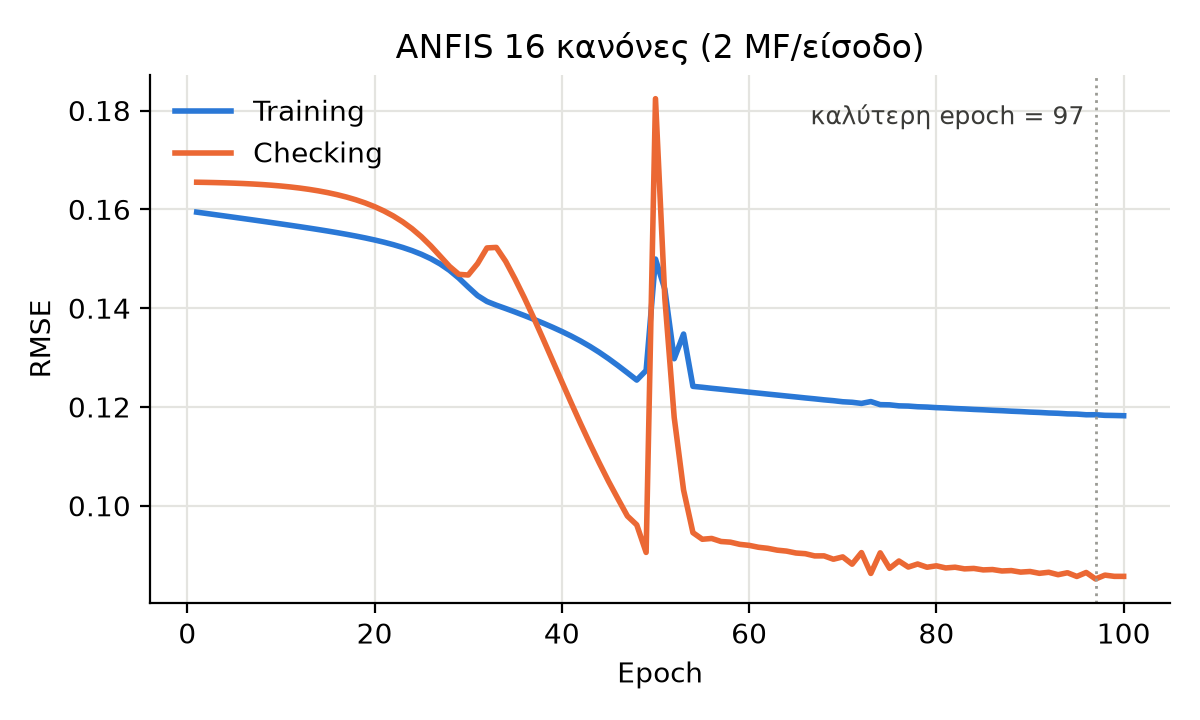
\includegraphics[width=\columnwidth]{errors_16rules.png}
\caption{RMSE σε Training και Checking ανά εποχή, για το μοντέλο των 16 κανόνων.
Η κατακόρυφη γραμμή σημειώνει την εποχή που επιλέχθηκε.}
\label{fig:err16}
\end{figure}

Για σύγκριση εκπαιδεύτηκε με τις ίδιες ρυθμίσεις και ένα μοντέλο με $M=3$ (81
κανόνες, 429 παράμετροι). Η εικόνα του (Σχ.~\ref{fig:err81}) είναι χαρακτηριστική
υπερπροσαρμογής. Το σφάλμα Training μειώνεται συνεχώς, μέχρι 0.06. Το σφάλμα
Checking έχει ελάχιστο 0.106 στην εποχή 11 και μετά τριπλασιάζεται. Χωρίς την
επιλογή εποχής βάσει Checking, το τελικό μοντέλο θα είχε περίπου τριπλάσιο σφάλμα
Checking.

\begin{figure}[!t]
\centering
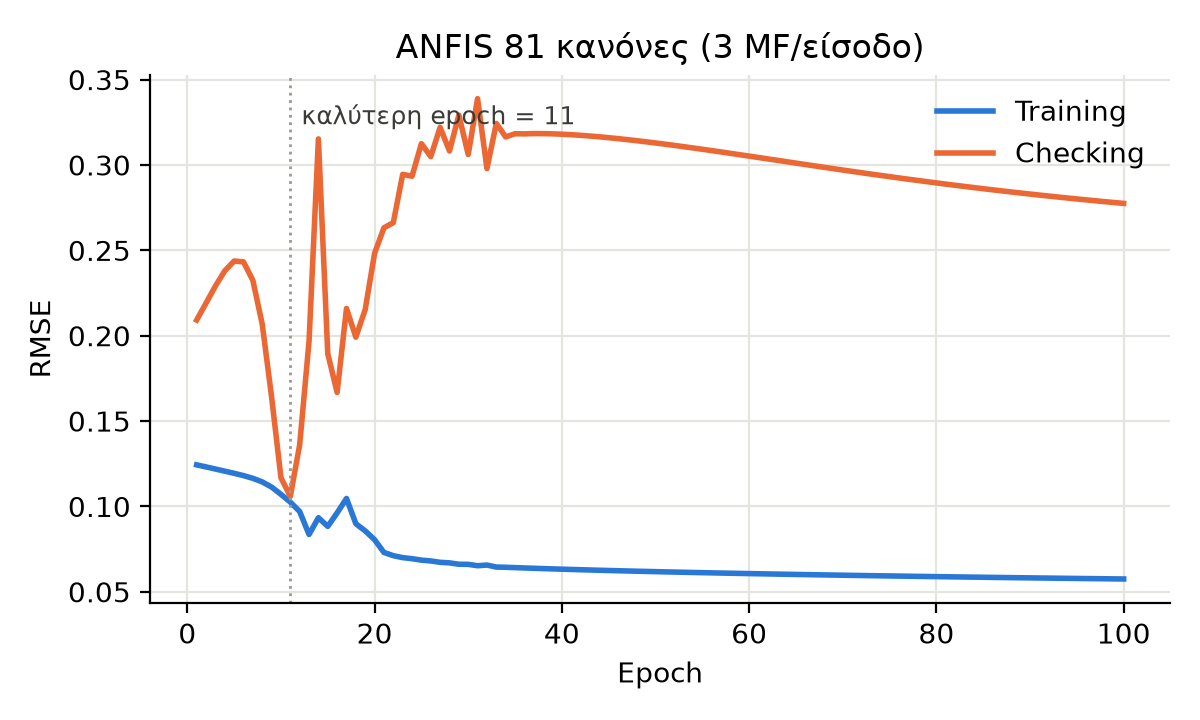
\includegraphics[width=\columnwidth]{errors_81rules.png}
\caption{RMSE ανά εποχή για το μοντέλο των 81 κανόνων: μετά την εποχή 11
το σφάλμα Checking αυξάνεται ενώ το σφάλμα Training μειώνεται (υπερπροσαρμογή).}
\label{fig:err81}
\end{figure}

\subsection{Συναρτήσεις συμμετοχής}
Το Σχ.~\ref{fig:mfs} συγκρίνει τις συναρτήσεις συμμετοχής πριν και μετά την
εκπαίδευση. Στις τρεις πρώτες εισόδους οι αλλαγές είναι μικρές. Στο
πλάτος πετάλου, το πιο διακριτικό χαρακτηριστικό του IRIS, οι καμπύλες
στένεψαν σημαντικά: τα $\sigma$ μειώθηκαν από 1.20 σε 0.39 και 0.26. Επίσης,
τα κέντρα μετακινήθηκαν λίγο έξω από το εύρος των δεδομένων (στα $-0.04$ και $2.82$ cm).
Για τιμές περίπου 1.2--2.0 cm και οι δύο βαθμοί συμμετοχής είναι μικροί. Λόγω όμως
της κανονικοποίησης \eqref{eq:wn} μετράει ο λόγος τους, ο οποίος μεταβάλλεται
απότομα, όπως μια σιγμοειδής συνάρτηση. Το σημείο όπου οι δύο κανονικοποιημένοι βαθμοί
γίνονται ίσοι βρίσκεται στα $1.675$ cm. Στα $1.5$ cm ο όρος «μεγάλο» έχει σχετικό
βάρος μόλις $0.6\%$, ενώ στα $1.8$ cm φτάνει το $97\%$. Η εκπαίδευση
δημιούργησε επομένως απότομο όριο στο χαρακτηριστικό που διαχωρίζει καλύτερα τις κλάσεις.
Το τίμημα είναι μικρότερη λεκτική ερμηνευσιμότητα των όρων «μικρό/μεγάλο» για
τη συγκεκριμένη είσοδο.

\begin{figure*}[!t]
\centering
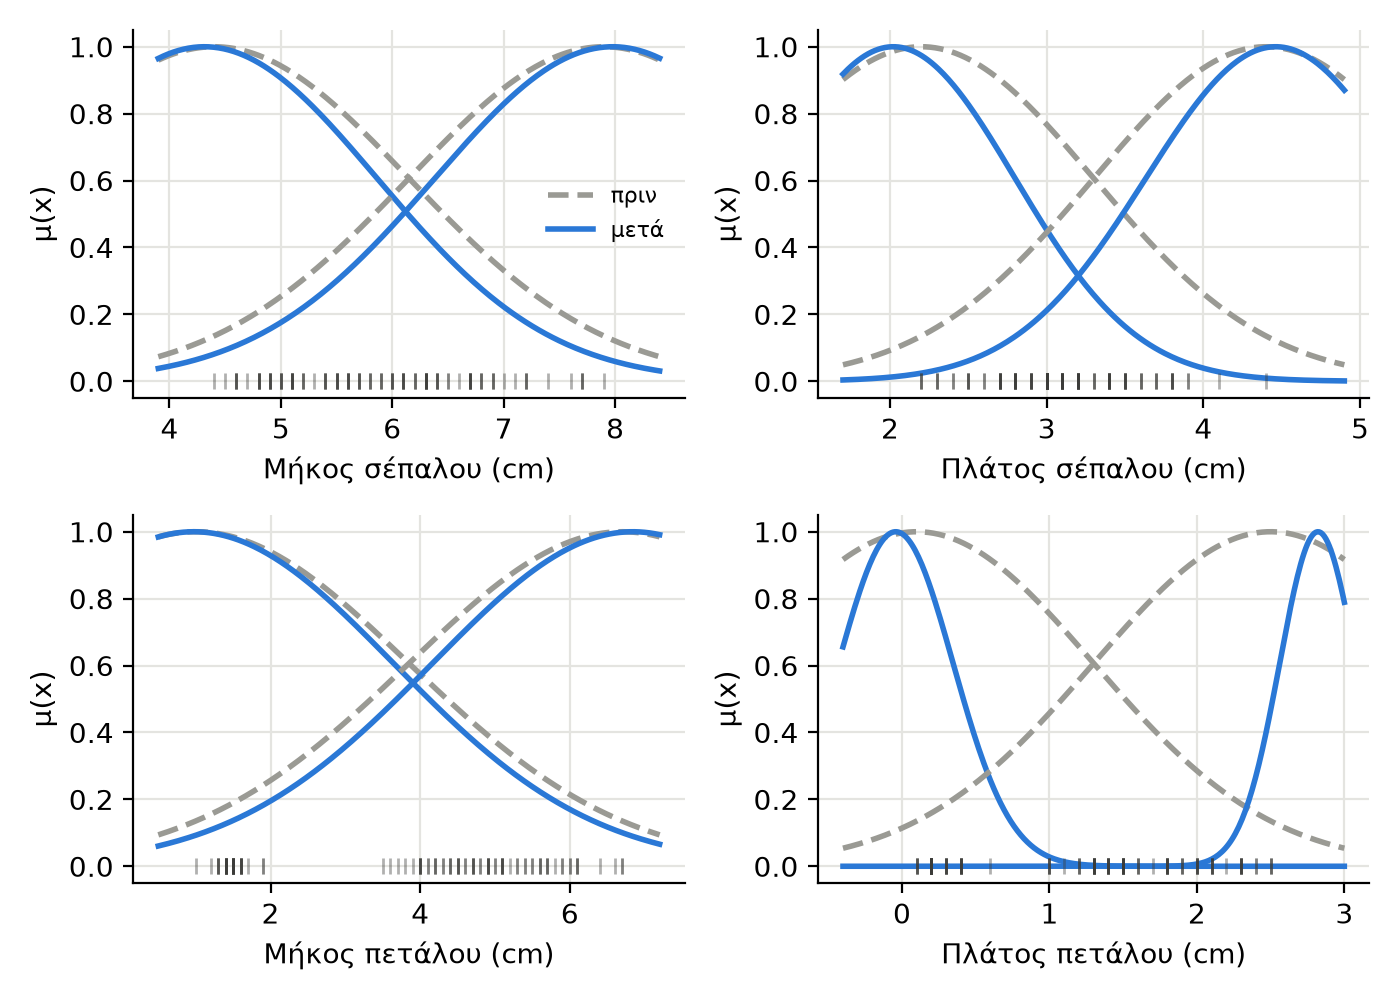
\includegraphics[width=0.75\textwidth]{mfs_16rules.png}
\caption{Gaussian συναρτήσεις συμμετοχής των τεσσάρων εισόδων πριν (διακεκομμένες)
και μετά (συνεχείς) την εκπαίδευση, για το μοντέλο των 16 κανόνων. Οι κατακόρυφες
γραμμές στον άξονα $x$ δείχνουν τα δείγματα Training.}
\label{fig:mfs}
\end{figure*}

\subsection{Αξιολόγηση στο Testing}
Το μοντέλο των 16 κανόνων ταξινόμησε σωστά 22 από τα 23 δείγματα του Testing,
δηλαδή ακρίβεια 95.65\%. Ο πίνακας σύγχυσης (Σχ.~\ref{fig:cm}) δείχνει ότι
η setosa και η virginica αναγνωρίστηκαν πλήρως και ότι το μοναδικό λάθος είναι μια
versicolor που ταξινομήθηκε ως virginica.

\begin{figure}[!t]
\centering
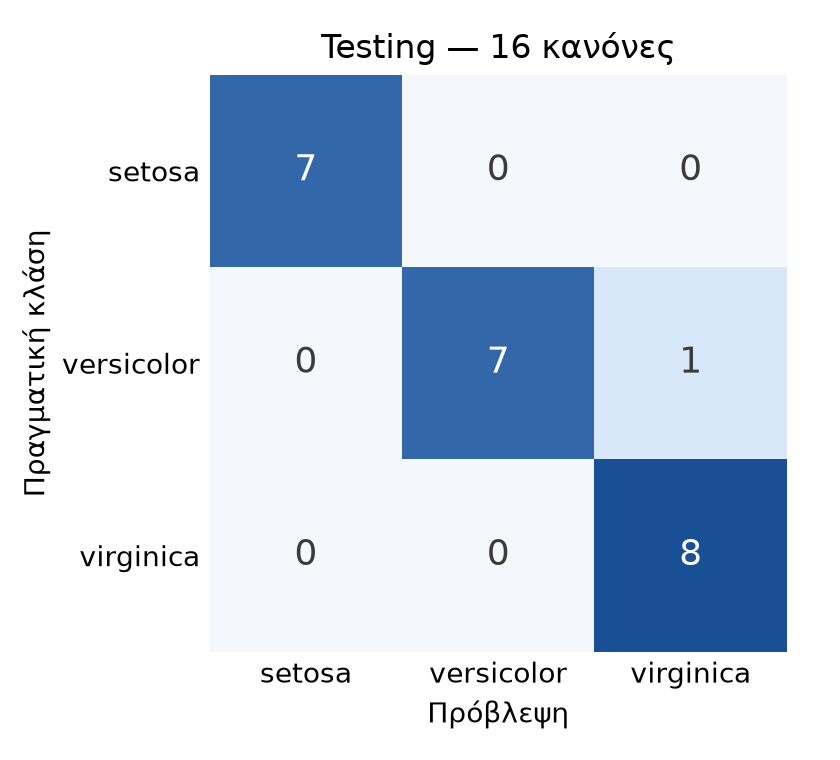
\includegraphics[width=0.78\columnwidth]{confusion_16rules.png}
\caption{Πίνακας σύγχυσης στο Testing (16 κανόνες). Γραμμές: πραγματική κλάση,
στήλες: πρόβλεψη.}
\label{fig:cm}
\end{figure}

Το Σχ.~\ref{fig:out} δείχνει την αριθμητική έξοδο κάθε δείγματος Testing μαζί με τα
όρια απόφασης. Οι έξοδοι σχηματίζουν τρεις σαφείς ομάδες:
\begin{itemize}
\item setosa: 0.91--1.08, δηλαδή τουλάχιστον 0.42 κάτω από το όριο 1.5·
\item versicolor: 1.97--2.15, για τα σωστά ταξινομημένα δείγματα·
\item virginica: 2.78--3.05.
\end{itemize}
Το περιθώριο μεταξύ versicolor και virginica είναι εμφανώς στενότερο από αυτό μεταξύ
setosa και versicolor.

\begin{figure}[!t]
\centering
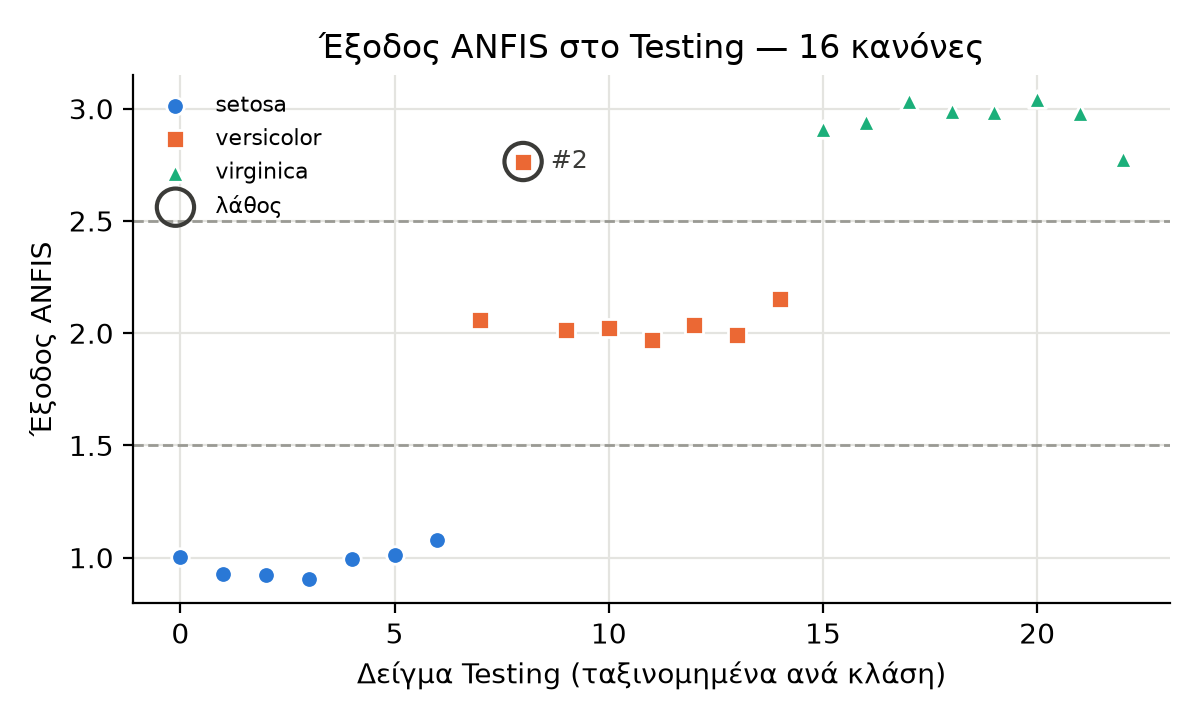
\includegraphics[width=\columnwidth]{outputs_16rules.png}
\caption{Αριθμητική έξοδος του ANFIS (16 κανόνες) για τα δείγματα Testing,
ταξινομημένα ανά πραγματική κλάση. Οι διακεκομμένες γραμμές είναι τα όρια
απόφασης 1.5 και 2.5· ο κύκλος σημειώνει τη λάθος ταξινόμηση.}
\label{fig:out}
\end{figure}

\subsection{Σύγκριση μοντέλων}
Ο Πίνακας~\ref{tab:compare} συγκρίνει τα τρία μοντέλα. Και τα τρία πέτυχαν την
ίδια ακρίβεια στο Testing και έκαναν το ίδιο λάθος. Το μοντέλο των 81 κανόνων έχει
4.5 φορές περισσότερες παραμέτρους, μεγαλύτερο σφάλμα Checking και ένα λάθος
περισσότερο στο Training. Το σχήμα one-vs-rest χρειάζεται τριπλάσιες παραμέτρους
για το ίδιο αποτέλεσμα. Με βάση την αρχή της απλούστερης επαρκούς λύσης, ως
τελικό μοντέλο επιλέγεται εκείνο των 16 κανόνων.

\begin{table}[!t]
\centering
\caption{Σύγκριση μοντέλων (ακρίβεια σε \%)}
\label{tab:compare}
\setlength{\tabcolsep}{4pt}
\begin{tabular}{lcccc}
\toprule
Μοντέλο & Παράμ. & Training & Checking & Testing \\
\midrule
ANFIS, 16 κανόνες & 96  & 99.04 & 100 & \textbf{95.65} \\
ANFIS, 81 κανόνες & 429 & 98.08 & 100 & 95.65 \\
3$\times$ANFIS one-vs-rest & 288 & 99.04 & 100 & 95.65 \\
\bottomrule
\end{tabular}
\end{table}

% ---------------------------------------------------------------------
\section{Παράδειγμα υπολογισμού βήμα προς βήμα}\label{sec:example}

Για να φανεί πώς το εκπαιδευμένο μοντέλο φτάνει σε μια απόφαση, ακολουθεί
ο υπολογισμός όλων των στρωμάτων για δύο δείγματα του Testing:
\begin{itemize}
\item Δείγμα Α, $\mathbf{x}=(5.6,\,2.5,\,3.9,\,1.1)$, μια versicolor
που ταξινομήθηκε σωστά·
\item Δείγμα Β, $\mathbf{x}=(6.7,\,3.0,\,5.0,\,1.7)$, η versicolor που
ταξινομήθηκε λάθος.
\end{itemize}
Στους πίνακες χρησιμοποιούνται οι συντομογραφίες ΜΣ/ΠΣ (μήκος/πλάτος σέπαλου),
ΜΠ/ΠΠ (μήκος/πλάτος πετάλου), καθώς και «μικ»/«μεγ» για τους όρους «μικρό»/«μεγάλο».

\subsection{Στρώμα 1: βαθμοί συμμετοχής}
Ο Πίνακας~\ref{tab:mu} δίνει τους βαθμούς συμμετοχής \eqref{eq:mf} των δύο δειγμάτων.
Στο δείγμα Α το πλάτος πετάλου (1.1 cm) είναι σαφώς «μικρό»: ο λόγος
$\mu_{\text{μεγ}}/\mu_{\text{μικ}}$ είναι της τάξης του $10^{-8}$. Στο δείγμα Β και οι δύο βαθμοί
του πλάτους πετάλου (1.7 cm) είναι πολύ μικροί, όμως ο «μεγάλος» είναι
διπλάσιος από τον «μικρό». Μετά την κανονικοποίηση αυτό σημαίνει περίπου
$67\%$ «μεγάλο», αφού το 1.7 βρίσκεται μόλις πάνω από το όριο των 1.675 cm.

\begin{table}[!t]
\centering
\caption{Βαθμοί συμμετοχής των δειγμάτων Α και Β (Στρώμα 1)}
\label{tab:mu}
\setlength{\tabcolsep}{4pt}
\begin{tabular}{lcccccc}
\toprule
 & \multicolumn{3}{c}{Δείγμα Α} & \multicolumn{3}{c}{Δείγμα Β} \\
\cmidrule(lr){2-4}\cmidrule(lr){5-7}
Είσοδος & $x$ & $\mu_{\text{μικ}}$ & $\mu_{\text{μεγ}}$ & $x$ & $\mu_{\text{μικ}}$ & $\mu_{\text{μεγ}}$ \\
\midrule
ΜΣ & 5.6 & 0.709 & 0.330 & 6.7 & 0.306 & 0.726 \\
ΠΣ & 2.5 & 0.827 & 0.061 & 3.0 & 0.453 & 0.212 \\
ΜΠ & 3.9 & 0.549 & 0.547 & 5.0 & 0.321 & 0.789 \\
ΠΠ & 1.1 & 0.014 & $3{\cdot}10^{-10}$ & 1.7 & $4.5{\cdot}10^{-5}$ & $9.1{\cdot}10^{-5}$ \\
\bottomrule
\end{tabular}
\end{table}

\subsection{Στρώματα 2--5: κανόνες και έξοδος}
Ο Πίνακας~\ref{tab:rules} δείχνει τους τέσσερις ισχυρότερους κανόνες για κάθε
δείγμα: την κανονικοποιημένη ισχύ τους $\bar w_k$ \eqref{eq:wn}, το
συμπέρασμά τους $f_k$ \eqref{eq:rule} και τη συνεισφορά τους $\bar w_k f_k$ στην
έξοδο \eqref{eq:out}.

\begin{table}[!t]
\centering
\caption{Οι τέσσερις ισχυρότεροι κανόνες για τα δείγματα Α και Β (Στρώματα 2--5)}
\label{tab:rules}
\setlength{\tabcolsep}{3.5pt}
\begin{tabular}{ccccccc}
\toprule
ΜΣ & ΠΣ & ΜΠ & ΠΠ & $\bar w_k$ & $f_k$ & $\bar w_k f_k$ \\
\midrule
\multicolumn{7}{l}{\textit{Δείγμα Α}: έξοδος $y=2.016\Rightarrow$ versicolor} \\
μικ & μικ & μικ & μικ & 0.318 & 4.052 & 1.289 \\
μικ & μικ & μεγ & μικ & 0.317 & 0.358 & 0.114 \\
μεγ & μικ & μικ & μικ & 0.148 & 1.821 & 0.270 \\
μεγ & μικ & μεγ & μικ & 0.148 & 1.554 & 0.230 \\
\multicolumn{4}{l}{υπόλοιποι 12 κανόνες} & 0.069 & --- & 0.114 \\
\midrule
\multicolumn{7}{l}{\textit{Δείγμα Β}: έξοδος $y=2.765\Rightarrow$ virginica} \\
μεγ & μικ & μεγ & μεγ & 0.228 & 2.866 & 0.654 \\
μεγ & μικ & μεγ & μικ & 0.113 & 2.380 & 0.269 \\
μεγ & μεγ & μεγ & μεγ & 0.107 & 1.448 & 0.154 \\
μικ & μικ & μεγ & μεγ & 0.096 & 2.324 & 0.223 \\
\multicolumn{4}{l}{υπόλοιποι 12 κανόνες} & 0.456 & --- & 1.465 \\
\bottomrule
\end{tabular}
\end{table}

Στο δείγμα Α όλοι οι ισχυροί κανόνες έχουν «ΠΠ μικρό», και οι τέσσερις πρώτοι
συγκεντρώνουν το $93\%$ του συνολικού βάρους. Το άθροισμα των συνεισφορών δίνει
$y=2.016$, πολύ κοντά στον στόχο 2. Τα επιμέρους $f_k$, όπως το $4.052$ του
πρώτου κανόνα, είναι τιμές τοπικών γραμμικών συναρτήσεων και αποκτούν νόημα μόνο
μέσα από τον σταθμισμένο συνδυασμό τους. Στα μοντέλα TSK πρώτης τάξης η ακρίβεια
αποκτάται συχνά σε βάρος της ερμηνευσιμότητας των μεμονωμένων κανόνων.

Στο δείγμα Β ο ισχυρότερος κανόνας είναι
«ΑΝ ΜΣ μεγάλο ΚΑΙ ΠΣ μικρό ΚΑΙ ΜΠ μεγάλο ΚΑΙ ΠΠ μεγάλο», με $f=2.866$, τιμή
κοντά στην κλάση virginica. Το βάρος είναι πιο μοιρασμένο: οι τέσσερις πρώτοι
κανόνες έχουν μόλις το $54\%$, επειδή κανένα χαρακτηριστικό δεν είναι ξεκάθαρα
«μικρό» ή «μεγάλο». Το τελικό $y=2.765$ ξεπερνά το όριο 2.5 και οδηγεί σε
virginica. Τα αίτια του λάθους εξετάζονται στην επόμενη ενότητα.

% ---------------------------------------------------------------------
\section{Σχολιασμός των λάθος ταξινομήσεων}

\subsection{Το λάθος στο Testing}
Το μοναδικό λάθος στο Testing είναι το δείγμα $\mathbf{x}=(6.7,\,3.0,\,5.0,\,1.7)$.
Ανήκει στην κλάση versicolor, αλλά το μοντέλο έδωσε έξοδο $y=2.765$,
0.265 πάνω από το όριο 2.5, και το ταξινόμησε ως virginica. Η εξέταση των
χαρακτηριστικών του δείχνει ότι το λάθος είναι εύλογο (Πίνακας~\ref{tab:err}):
\begin{itemize}
\item Το μήκος πετάλου (5.0 cm) είναι πολύ πάνω από τον μέσο όρο της versicolor
(4.33) και πιο κοντά σε αυτόν της virginica (5.58).
\item Το πλάτος πετάλου (1.7 cm) είναι από τις μεγαλύτερες τιμές της versicolor
στο Training (μέγιστο 1.8), ενώ για τη virginica είναι συνηθισμένη τιμή
(εύρος 1.5--2.5).
\item Το μήκος σέπαλου (6.7 cm) σχεδόν συμπίπτει με τον μέσο όρο της virginica (6.64).
\item Η ευκλείδεια απόσταση του δείγματος από τον μέσο όρο της virginica (0.68)
είναι μικρότερη από ό,τι από τον μέσο όρο της δικής του κλάσης (1.03).
\end{itemize}
Με βάση τα τέσσερα χαρακτηριστικά του, το δείγμα βρίσκεται μέσα στην περιοχή
της virginica, στη ζώνη όπου οι κλάσεις versicolor και virginica του IRIS
επικαλύπτονται.

Η Ενότητα~\ref{sec:example} δείχνει πώς προκύπτει το λάθος. Το μοντέλο
έμαθε ένα όριο στο πλάτος πετάλου στα $1.675$ cm, και το δείγμα (1.7 cm)
βρίσκεται μόλις $0.025$ cm πάνω από αυτό. Έτσι ενεργοποιούνται κυρίως κανόνες
με «ΠΠ μεγάλο». Το όριο είναι λογικό με βάση τα δεδομένα εκπαίδευσης: μόνο 3 από τις
34 versicolor του Training έχουν πλάτος πετάλου $\ge1.6$ cm, ενώ το ίδιο ισχύει για
33 από τις 35 virginica.

\begin{table}[!t]
\centering
\caption{Το λάθος δείγμα σε σύγκριση με τους μέσους όρους των κλάσεων στο Training (cm)}
\label{tab:err}
\setlength{\tabcolsep}{4pt}
\begin{tabular}{lcccc}
\toprule
 & $x_1$ & $x_2$ & $x_3$ & $x_4$ \\
\midrule
Λάθος δείγμα (versicolor) & 6.70 & 3.00 & 5.00 & 1.70 \\
Μέσος όρος versicolor     & 6.04 & 2.79 & 4.33 & 1.34 \\
Μέσος όρος virginica      & 6.64 & 3.05 & 5.58 & 2.05 \\
\bottomrule
\end{tabular}
\end{table}

\subsection{Το λάθος είναι ανεξάρτητο από το μοντέλο}
Και τα τρία μοντέλα του Πίνακα~\ref{tab:compare} ταξινόμησαν λάθος το ίδιο δείγμα.
Το μοντέλο των 81 κανόνων έδωσε $y=2.605$, πιο κοντά στο όριο αλλά ακόμη πάνω από αυτό.
Το σχήμα one-vs-rest δεν υποθέτει διάταξη των κλάσεων. Οι έξοδοι των τριών εξειδικευμένων ANFIS ήταν
0.00 (setosa), 0.28 (versicolor) και 0.72 (virginica). Η έξοδος του μοντέλου
της virginica είναι η μεγαλύτερη, με σαφή διαφορά από της versicolor. Αυτό αποκλείει την
κωδικοποίηση 1/2/3 ως αιτία του λάθους και ενισχύει το συμπέρασμα ότι το λάθος οφείλεται
στα δεδομένα.

\subsection{Λάθη στο Training}
Στο Training το κύριο μοντέλο έκανε επίσης ένα μόνο λάθος, στην αντίθετη
κατεύθυνση: μια virginica $(6.3,\,2.8,\,5.1,\,1.5)$ με έξοδο 2.409 ταξινομήθηκε ως
versicolor, 0.09 κάτω από το όριο. Το δείγμα αυτό έχει το μικρότερο πλάτος
πετάλου που εμφανίζει η virginica (1.5 cm). Η τιμή αυτή βρίσκεται κάτω από το
όριο των 1.675 cm, όπου ο όρος «ΠΠ μεγάλο» έχει σχετικό βάρος μόλις $0.6\%$.
Πρόκειται για το συμμετρικό λάθος του δείγματος Β. Το μοντέλο των 81 κανόνων έκανε το ίδιο λάθος
και ένα επιπλέον, μια versicolor $(6.0,\,2.7,\,5.1,\,1.6)$ με έξοδο 2.502, ουσιαστικά
πάνω στο όριο. Όλα τα λάθη, σε όλα τα σύνολα και σε όλα τα μοντέλα, αφορούν
το ζεύγος versicolor/virginica. Η setosa δεν μπερδεύτηκε ποτέ, πράγμα αναμενόμενο
αφού είναι γραμμικά διαχωρίσιμη.

% ---------------------------------------------------------------------
\section{Συζήτηση και περιορισμοί}

\textit{Μέγεθος συνόλων.} Με 23 δείγματα στο Testing, κάθε λάθος μεταβάλλει την
ακρίβεια κατά 4.35 ποσοστιαίες μονάδες. Η εκτίμηση 95.65\% έχει επομένως
σημαντική αβεβαιότητα. Η διασταυρωμένη επικύρωση (k-fold cross-validation) θα
έδινε πιο σταθερή εκτίμηση, αλλά ξεφεύγει από το ζητούμενο σχήμα
Training/Checking/Testing.

\textit{Σφάλμα Checking μικρότερο από Training.} Στο κύριο μοντέλο το RMSE
Checking (0.085) βγήκε μικρότερο από το RMSE Training (0.118). Αυτό δεν
είναι ένδειξη λάθους. Το Checking έχει μόνο 23 δείγματα και, λόγω της τυχαίας
δειγματοληψίας, περιέχει λιγότερα «δύσκολα» δείγματα της ζώνης επικάλυψης.
Επιπλέον, επειδή η εποχή επιλέχθηκε με βάση το Checking, το σφάλμα του είναι
ελαφρά αισιόδοξο. Για τον λόγο αυτό η τελική αξιολόγηση γίνεται αποκλειστικά στο
ανεξάρτητο Testing.

\textit{Αριθμός κανόνων.} Η διαμέριση πλέγματος οδηγεί σε $M^n$ κανόνες, πλήθος
που αυξάνεται εκθετικά με τις εισόδους. Ήδη για $M=3$ οι παράμετροι
συμπεράσματος (405) ξεπερνούν κατά πολύ τα δείγματα (104), και το μοντέλο
γίνεται επιρρεπές σε υπερπροσαρμογή, όπως φάνηκε στο Σχ.~\ref{fig:err81}.
Εναλλακτικές μέθοδοι δημιουργίας κανόνων, όπως η αφαιρετική ομαδοποίηση
(subtractive clustering), θα μπορούσαν να δώσουν λιγότερους και πιο στοχευμένους
κανόνες.

\textit{Υλοποίηση.} Η αριθμητική κλίση είναι απλή και εύκολα επαληθεύσιμη, αλλά το
κόστος της αυξάνεται γραμμικά με το πλήθος των παραμέτρων υπόθεσης. Για
μεγαλύτερα προβλήματα θα ήταν προτιμότερες οι αναλυτικές παράγωγοι ή η αυτόματη
παραγώγιση.

% ---------------------------------------------------------------------
\section{Συμπεράσματα}

Υλοποιήθηκε από την αρχή ένα ANFIS τύπου TSK πρώτης τάξης με 16 κανόνες. Η εκπαίδευση
ήταν υβριδική, με ελάχιστα τετράγωνα με ridge για τα συμπεράσματα και κατάβαση
αριθμητικής κλίσης για τις συναρτήσεις συμμετοχής. Η επιλογή της εποχής έγινε βάσει
του συνόλου Checking. Ως ταξινομητής για το IRIS, με αντιστοίχιση εξόδου σε κλάση
μέσω στρογγυλοποίησης και αποκοπής, πέτυχε ακρίβεια 95.65\% στο ανεξάρτητο
σύνολο Testing. Η κανονικοποίηση ridge αποδείχθηκε απαραίτητη για τον περιορισμό
της υπερπροσαρμογής, και η επιλογή εποχής βάσει Checking ήταν κρίσιμη για το
μεγαλύτερο μοντέλο των 81 κανόνων. Το μοναδικό λάθος ταξινόμησης αφορά ένα
δείγμα versicolor που βρίσκεται μέσα στην περιοχή της virginica. Το ότι το ίδιο λάθος
κάνουν τρεις διαφορετικές αρχιτεκτονικές δείχνει ότι πρόκειται για εγγενή
δυσκολία των δεδομένων. Ως μελλοντική εργασία προτείνονται η διασταυρωμένη
επικύρωση, η δημιουργία κανόνων με ομαδοποίηση και η μελέτη μοντέλων με
μόνο τα δύο χαρακτηριστικά του πετάλου.

% ---------------------------------------------------------------------
\section*{Δήλωση χρήσης εργαλείων τεχνητής νοημοσύνης}
Κατά την εκπόνηση της εργασίας χρησιμοποιήθηκε το εργαλείο τεχνητής νοημοσύνης
Claude (Anthropic) ως βοηθητικό μέσο, για υποστήριξη στη συγγραφή και στον έλεγχο
του κώδικα και για την επιμέλεια του κειμένου. Ο κώδικας και τα αποτελέσματα
ελέγχθηκαν από τον συγγραφέα, ο οποίος έχει την ευθύνη για το περιεχόμενο της εργασίας.

\begin{thebibliography}{99}

\bibitem{zadeh1965}
L.~A. Zadeh, ``Fuzzy sets,'' \textit{Information and Control}, vol.~8, no.~3,
pp.~338--353, 1965.

\bibitem{takagi1985}
T.~Takagi and M.~Sugeno, ``Fuzzy identification of systems and its applications
to modeling and control,'' \textit{IEEE Trans. Syst., Man, Cybern.}, vol.~SMC-15,
no.~1, pp.~116--132, 1985.

\bibitem{sugeno1988}
M.~Sugeno and G.~T. Kang, ``Structure identification of fuzzy model,''
\textit{Fuzzy Sets and Systems}, vol.~28, no.~1, pp.~15--33, 1988.

\bibitem{jang1993}
J.-S.~R. Jang, ``ANFIS: Adaptive-network-based fuzzy inference system,''
\textit{IEEE Trans. Syst., Man, Cybern.}, vol.~23, no.~3, pp.~665--685, 1993.

\bibitem{fisher1936}
R.~A. Fisher, ``The use of multiple measurements in taxonomic problems,''
\textit{Annals of Eugenics}, vol.~7, no.~2, pp.~179--188, 1936.

\bibitem{hoerl1970}
A.~E. Hoerl and R.~W. Kennard, ``Ridge regression: Biased estimation for
nonorthogonal problems,'' \textit{Technometrics}, vol.~12, no.~1, pp.~55--67, 1970.

\bibitem{matlab}
The MathWorks, Inc., \textit{Fuzzy Logic Toolbox User's Guide}. Natick, MA, USA.

\bibitem{numpy2020}
C.~R. Harris \textit{et al.}, ``Array programming with NumPy,''
\textit{Nature}, vol.~585, pp.~357--362, 2020.

\bibitem{sklearn2011}
F.~Pedregosa \textit{et al.}, ``Scikit-learn: Machine learning in Python,''
\textit{J. Mach. Learn. Res.}, vol.~12, pp.~2825--2830, 2011.

\bibitem{adamidis}
Π.~Αδαμίδης, \textit{Ευφυή Συστήματα — Σημειώσεις Ασαφών Συστημάτων}.
ΔΙΠΑΕ, 2025--26.

\end{thebibliography}

\end{document}
